\chapter{Konzept}

Zum Beispiel:  
- Blockbild der Architektur Ihrer Anwendung  
- Pseudocode für Algorithmen  
- mathematische Formeln  
- evtl. Diagramme auf hohem Abstraktionsniveau.  

\section{Grundkonzept}

	\paragraph{Der Telegram Bot als Herzstück}
 	Das Herzstück der Applikation ist der Telegram-Bot selbst. Er wird von einem Benutzer angesprochen und reagiert auf seine Eingabe. So können verschieden Funktionen ausgelöst werden. Bspw. werden Antworten zurückgegeben, Informationen gespeichert oder es wird ein Vorschlag gemacht und an den Nutzer zurückgegeben. Der Bot soll mit mehreren Benutzern gleichzeitig sprechen können. Das wird ermöglicht, weil alle Reaktionen des Bots mit der Kennung des einzelnen Nutzers verbunden sind. So spricht der Bot den Nutzer mit Namen an oder kann sich daran erinnnern, welche Fragen schon beantwortet wurden und welche nicht. 
	 
	 


 \begin{figure} %[hbtp]
	\centering
	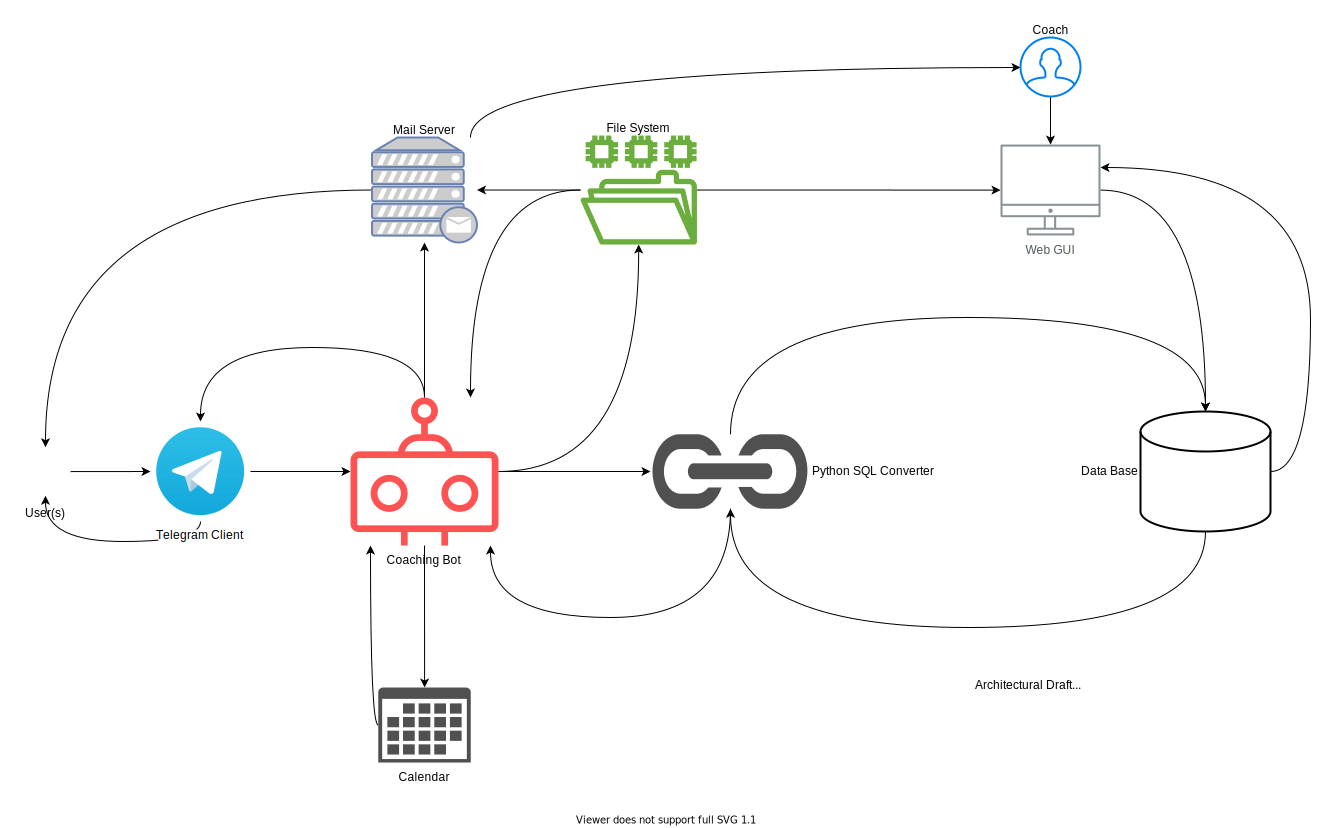
\includegraphics{concept and fancy drawings/PA_Architecture.svg}
	\caption{Architektur für das Projekt "Der Coaching Bot" auf hohem Abstraktionsniveau}
	\label{architecture}
\end{figure}


\begin{figure} %[hbtp]
	\centering
	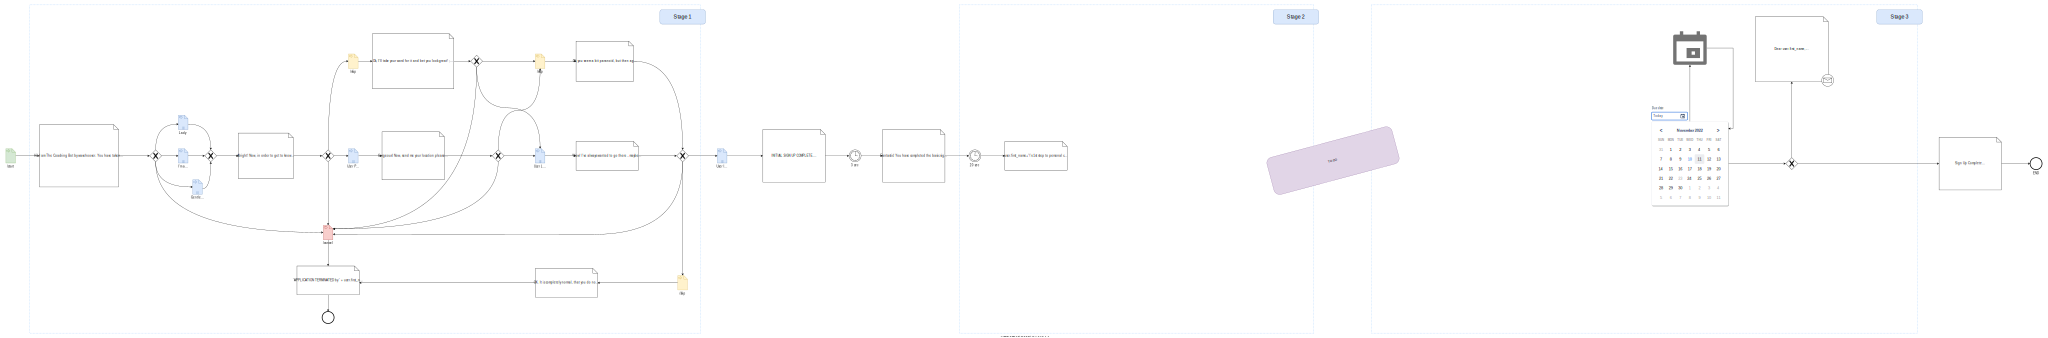
\includegraphics{concept and fancy drawings/PA_Conversation_Flow.svg}
	\caption{Konversationsfluss des Bots}
	\label{conversationFlow}
\end{figure}

